% THIS DOCUMENT IS FOLLOWS THE VOLERE TEMPLATE BY Suzanne Robertson and James Robertson
% ONLY THE SECTION HEADINGS ARE PROVIDED
%
% Initial draft from https://github.com/Dieblich/volere
%
% Risks are removed because they are covered by the Hazard Analysis
\documentclass[12pt]{article}

\usepackage{booktabs}
\usepackage{tabularx}
\usepackage{hyperref}
\usepackage{graphicx}

\hypersetup{
    bookmarks=true,         % show bookmarks bar?
      colorlinks=true,      % false: boxed links; true: colored links
    linkcolor=red,          % color of internal links (change box color with linkbordercolor)
    citecolor=green,        % color of links to bibliography
    filecolor=magenta,      % color of file links
    urlcolor=cyan           % color of external links
}

\newcommand{\lips}{\textit{Insert your content here.}}

%% Comments

\usepackage{color}

\newif\ifcomments\commentstrue %displays comments
%\newif\ifcomments\commentsfalse %so that comments do not display

\ifcomments
\newcommand{\authornote}[3]{\textcolor{#1}{[#3 ---#2]}}
\newcommand{\todo}[1]{\textcolor{red}{[TODO: #1]}}
\else
\newcommand{\authornote}[3]{}
\newcommand{\todo}[1]{}
\fi

\newcommand{\wss}[1]{\authornote{blue}{SS}{#1}} 
\newcommand{\plt}[1]{\authornote{magenta}{TPLT}{#1}} %For explanation of the template
\newcommand{\an}[1]{\authornote{cyan}{Author}{#1}}

%% Common Parts

\newcommand{\progname}{Software Engineering} % PUT YOUR PROGRAM NAME HERE
\newcommand{\authname}{Team 8 -- Rhythm Rangers\\
\\ Ansel Chen
\\ Muhammad Jawad
\\ Mohamad-Hassan Bahsoun
\\ Matthew Baleanu
\\ Ahmed Al-Hayali} % AUTHOR NAMES                  

\usepackage{hyperref}
    \hypersetup{colorlinks=true, linkcolor=blue, citecolor=blue, filecolor=blue,
                urlcolor=blue, unicode=false}
    \urlstyle{same}
                                


\begin{document}

\title{Software Requirements Specification for \progname: subtitle describing software} 
\author{\authname}
\date{\today}
	
\maketitle

~\newpage

\pagenumbering{roman}

\tableofcontents

~\newpage

\section*{Revision History}

\begin{tabularx}{\textwidth}{p{3cm}p{2cm}X}
\toprule {\textbf{Date}} & {\textbf{Version}} & {\textbf{Notes}}\\
\midrule
Date 1 & 1.0 & Notes\\
Date 2 & 1.1 & Notes\\
\bottomrule
\end{tabularx}

~\\

~\newpage
\section{Purpose of the Project}
\subsection{User Business}
\lips
\subsection{Goals of the Project}
\lips
\section{Stakeholders}
\subsection{Client}
\lips
\subsection{Customer}
\lips
\subsection{Other Stakeholders}
\lips
\subsection{Hands-On Users of the Project}
\lips
\subsection{Personas}
\lips
\subsection{Priorities Assigned to Users}
\lips
\subsection{User Participation}
\lips
\subsection{Maintenance Users and Service Technicians}
\lips

\section{Mandated Constraints}
\subsection{Solution Constraints}
\begin{itemize}

  \item The service uses a music dataset
  \\ \textbf{Rationale:} A dataset for an AI project is necessary as some form of training data must be used 
  in order to train the AI generative, analysis and recommendation systems. 
  \\ \textbf{Fit Criterion:} The machine learning algorithms use a music dataset as the training set. 

  \item The service uses a machine learning algorithm in order to generate song recommendations and snippets. 
  \\ \textbf{Rationale:} The general gist of this project is a leveraging of different signal processing and machine learning
  algorithms in order to provide an end user with a better experience for consuming music. We believe that using a machine 
  learning algorithm for these ends would both be interesting in terms of implementing and training a model, but also practically
  useful for the end user to provide better recommendations by leveraging training over a very large dataset in order to produce results. 
  \\\textbf{Fit Criterion:} The recommendation and generation components utilize trained machine learning algorithm. 

  \item The service features integration with an existing music streaming provider's platform. 
  \\ \textbf{Rationale:} A music service provider (such as Spotify) would allow the service to bypass the need to have
  music inputted, instead being able to use references to a track. In addition, through API calls, providers such as spotify
  already have a large amount of useful labels for invidiual track(s) that can be used as features for the machine learning
  components of the service.  
  \\ \textbf{Fit Criterion:} The service has components that make uses of features (such as API calls) 
  that belong to a music service provider's platform. 

  \item The service uses a server to process the user requests separately from the front end.
  \\ \textbf{Rationale:} Ideally, our service would use an on-premise deployed ubuntu server in order to process the user 
  analysis, recommendation, and generation components of the project, as this would allow a more flexible front end design
  (such as through a web application). 
  \\ \textbf{Fit Criterion:} An on-premise server is deployed for the purposes of handling the analysis, generation and recommendations
  systems separately from the front end. 

\end{itemize}

\subsection{Implementation Environment of the Current System}
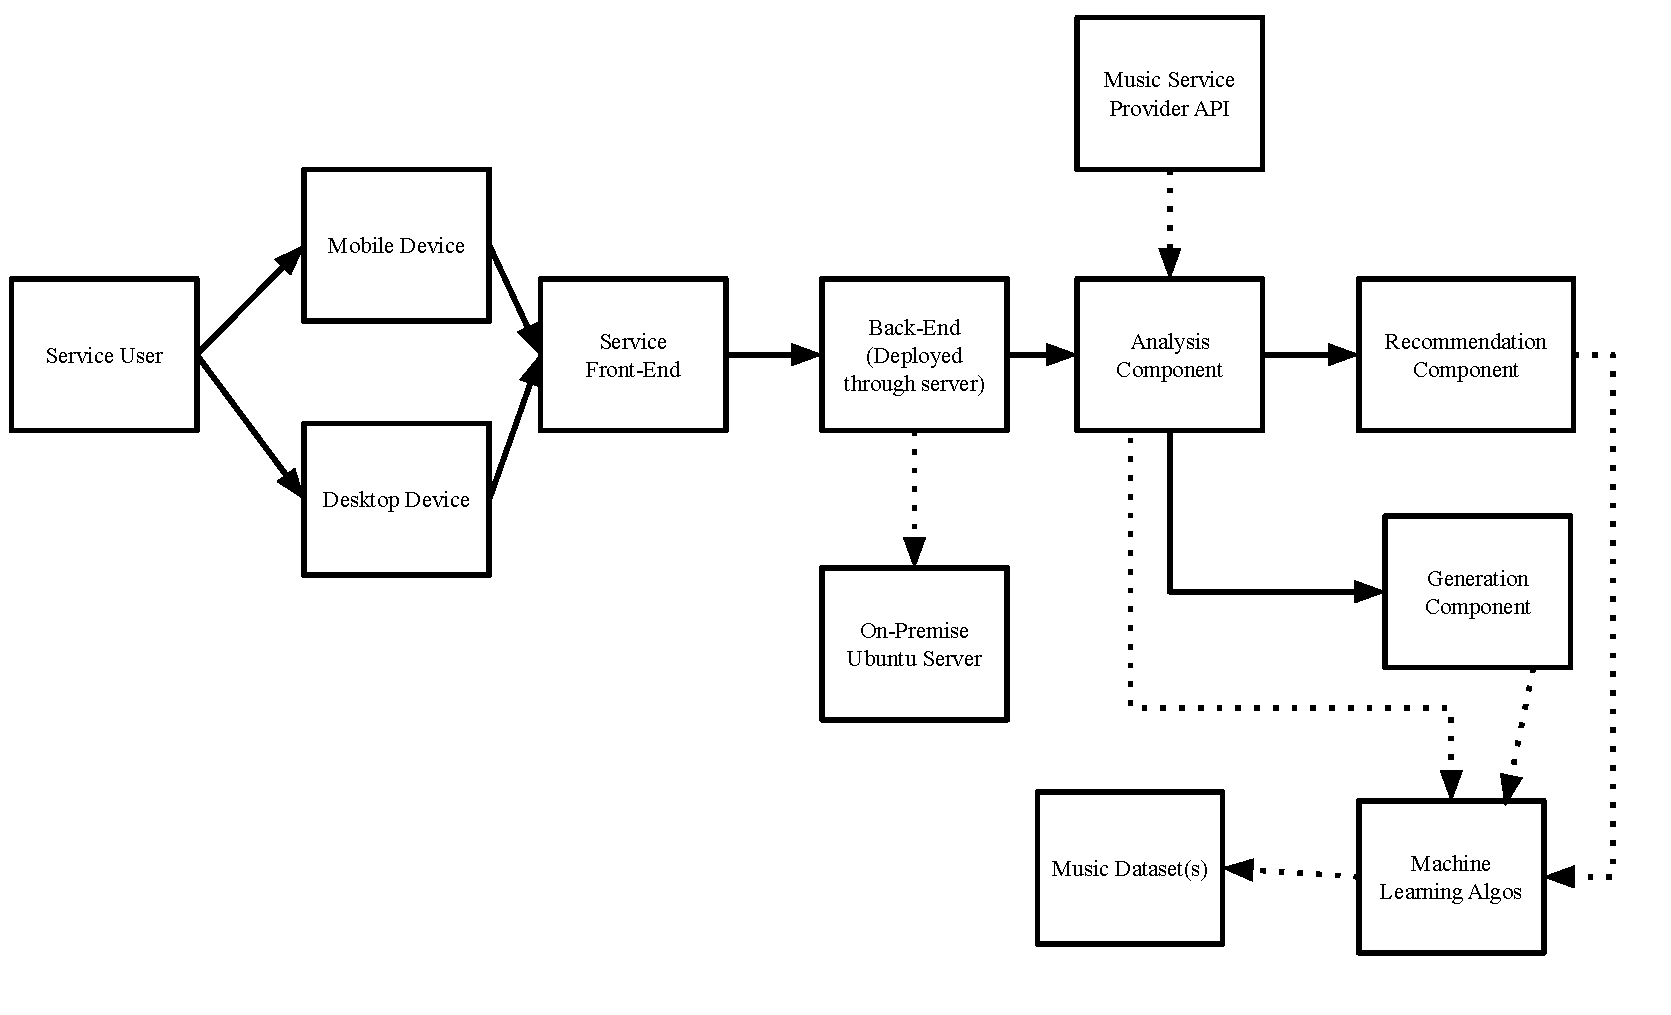
\includegraphics[scale=0.552]{3_2_environment_diagram.pdf}

\subsection{Partner or Collaborative Applications}
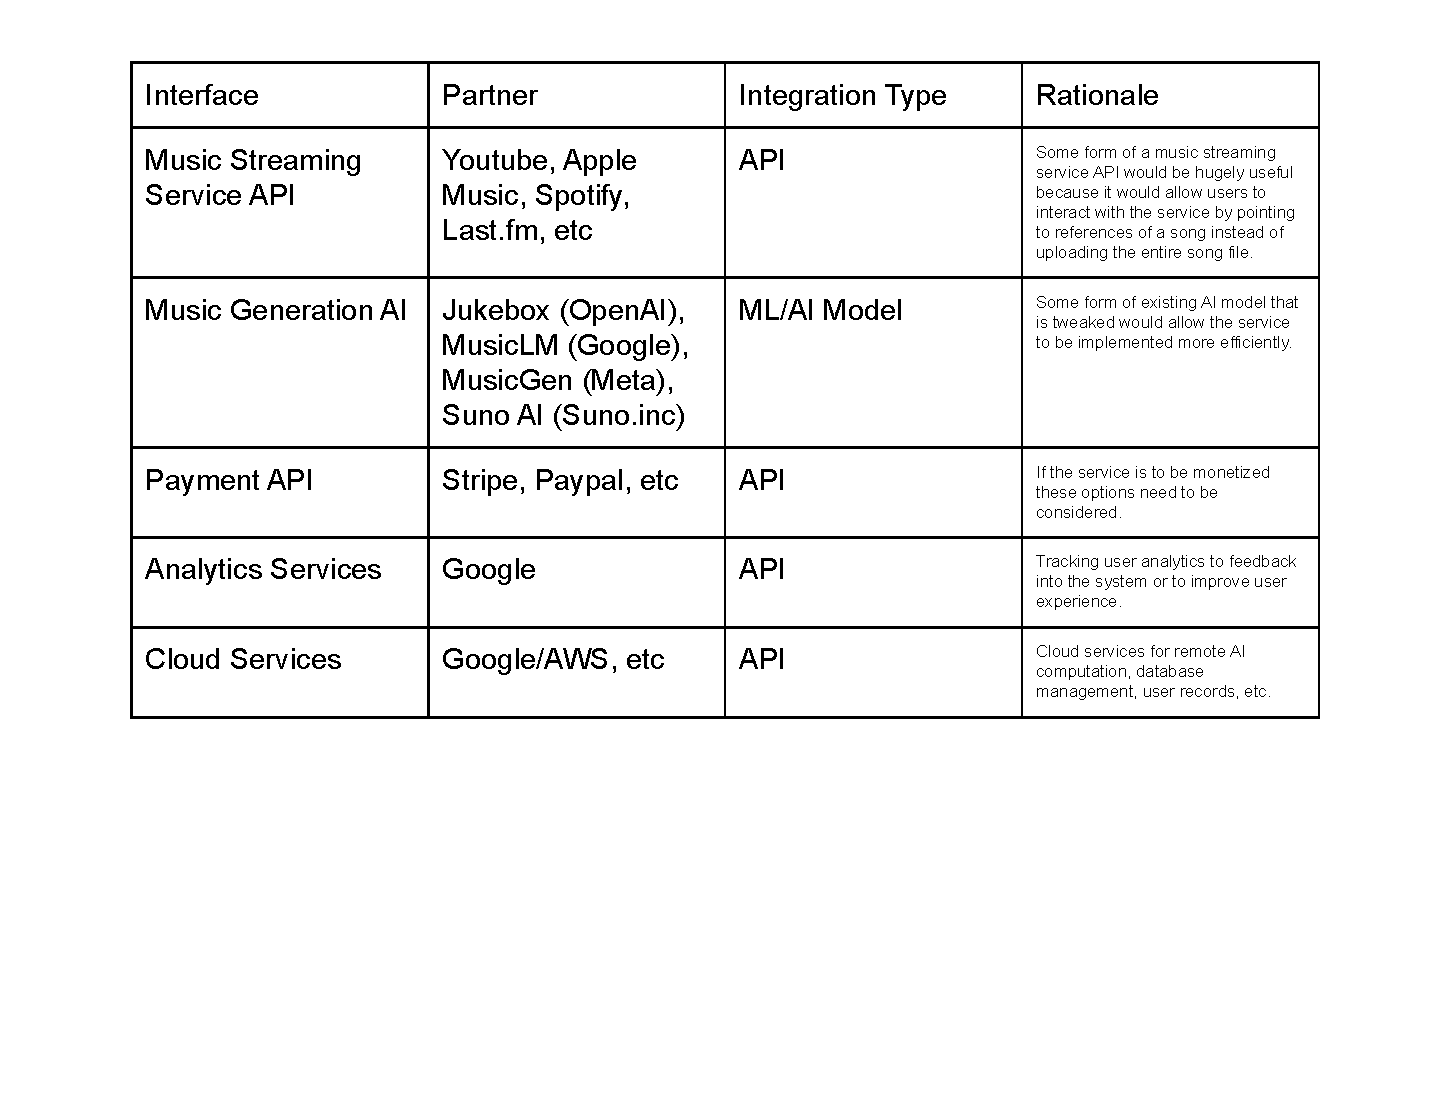
\includegraphics[scale=0.72]{3_3_partner_constraints_figure}

\subsection{Off-the-Shelf Software}
There are several existing solutions that could serve as part of the music generation and recommendation system. These include:

\begin{itemize}
    \item \textbf{Spotify API}: Provides access to a vast library of music, including song previews and metadata, which can be leveraged for generating recommendations.
    \item \textbf{Librosa Library}: An open-source Python package for analyzing and processing music files, suitable for extracting features from songs and facilitating generative components.
    \item \textbf{TensorFlow and PyTorch Pre-trained Models}: Both frameworks offer pre-trained models that could be adapted for music generation tasks. These solutions provide a basis for deep learning models without having to build and train from scratch.
    \item \textbf{OpenAI Jukebox}: A generative model that is capable of producing music, which could potentially be adapted and integrated into our system.
\end{itemize}

These off-the-shelf software solutions provide a foundation upon which we can build our custom features, significantly reducing the development time and leveraging existing technologies to enhance the functionality of our platform.

\subsection{Anticipated Workplace Environment}
\begin{itemize}
  \item Home Usage
  \\ \textbf{Rationale:} This environment is more appropriate for casual music listeners. 
  This means users will most likely be using it in a form of a casual environment, such as their phone.
  This means that uploading songs and snippets must be easy and convenient on a mobile device, such 
  as being able to directly input a spotify platlist. 

  \item Studio Usage
  \\ \textbf{Rationale:} This environment is more professional and what is most likely what 
  creative professionals will be using. The expectation is that they will be using this on their 
  computers, thus they are more likely have a reliable internet connection in addition to being
  willing to input a lot more music to the service. T

\end{itemize}

\subsection{Schedule Constraints}
This project was started in the 2024 Fall Term and is expected to be completed by the 
2025 winter term at McMaster university. Some of the key deadlines are: 
\begin{itemize}
  \item Proof of concept, November 11-22nd
  \\This deadline accounts for 5\% of the mark. This deadline involves having some form of a 
  working demo to show the project supervisors that some concrete development work has been done and 
  to reassess the feasibility of certain aspects of the project. If a working demonstration of the key 
  features of the project cannot be presented to the supervisor by this deadline, then most likely 
  certain currently planned features will have to be put on the cutting floor. 

  \item Proof of concept, November 11-22nd
  \\This deadline accounts for 20\% of the mark. This deadline involves a demonstration of a finalized 
  version of the project to supervisors before the public EXPO happening at a TBD date. By this deadline, 
  the service should be in a completed state ready for use and demonstration. If this deadline is not met then
  the project can be considered a "failure". 

  \item Final Documentation, April 2
  \\This deadline accounts for 30\% of the mark. It involves the finalized documentation of plans pertaining to 
  the project and the actual working program/service. Any final revisions and reflections pertaining to the project
  should have been completed by this deadline as no further changes to the project will be possible. Whatever documentation
  or code that is not completed by this deadline would be considered permanently unfinished. 
\end{itemize}

\subsection{Budget Constraints}
The budget limit as stated by the capstone outline is 750\$ CAD. Potential additional
costs might include API calls, software liscensing, account fees for cloud services. 
For the purposes of the demonstration they should not exceed the 750\$ limit. 

\subsection{Enterprise Constraints}
There are no specific enterprise constraints as we do not have outside investors
for this project. 

\section{Naming Conventions and Terminology}
\subsection{Glossary of All Terms, Including Acronyms, Used by Stakeholders
involved in the Project}
\lips

\section{Relevant Facts And Assumptions}
\subsection{Relevant Facts}
\lips
\subsection{Business Rules}
\lips
\subsection{Assumptions}
\lips

\section{The Scope of the Work}
\subsection{The Current Situation}
\lips
\subsection{The Context of the Work}
\lips
\subsection{Work Partitioning}
\lips
\subsection{Specifying a Business Use Case (BUC)}
\lips

\section{Business Data Model and Data Dictionary}
\subsection{Business Data Model}
\lips
\subsection{Data Dictionary}
\lips

\section{The Scope of the Product}
\subsection{Product Boundary}
\lips
\subsection{Product Use Case Table}
\lips
\subsection{Individual Product Use Cases (PUC's)}
\lips

\section{Functional Requirements}
\subsection{Functional Requirements}
\lips

\section{Look and Feel Requirements}
\subsection{Appearance Requirements}
\lips
\subsection{Style Requirements}
\lips

\section{Usability and Humanity Requirements}
\subsection{Ease of Use Requirements}
\lips
\subsection{Personalization and Internationalization Requirements}
\lips
\subsection{Learning Requirements}
\lips
\subsection{Understandability and Politeness Requirements}
\lips
\subsection{Accessibility Requirements}
\lips

\section{Performance Requirements}
\subsection{Speed and Latency Requirements}
\lips
\subsection{Safety-Critical Requirements}
\lips
\subsection{Precision or Accuracy Requirements}
\lips
\subsection{Robustness or Fault-Tolerance Requirements}
\lips
\subsection{Capacity Requirements}
\lips
\subsection{Scalability or Extensibility Requirements}
\lips
\subsection{Longevity Requirements}
\lips

\section{Operational and Environmental Requirements}
\subsection{Expected Physical Environment}
\lips
\subsection{Wider Environment Requirements}
\lips
\subsection{Requirements for Interfacing with Adjacent Systems}
\lips
\subsection{Productization Requirements}
\lips
\subsection{Release Requirements}
\lips

\section{Maintainability and Support Requirements}
\subsection{Maintenance Requirements}
\lips
\subsection{Supportability Requirements}
\lips
\subsection{Adaptability Requirements}
\lips

\section{Security Requirements}
\subsection{Access Requirements}
\lips
\subsection{Integrity Requirements}
\lips
\subsection{Privacy Requirements}
\lips
\subsection{Audit Requirements}
\lips
\subsection{Immunity Requirements}
\lips

\section{Cultural Requirements}
\subsection{Cultural Requirements}
\lips

\section{Compliance Requirements}
\subsection{Legal Requirements}
\lips
\subsection{Standards Compliance Requirements}
\lips

\section{Open Issues}
\lips

\section{Off-the-Shelf Solutions}
\subsection{Ready-Made Products}
\lips
\subsection{Reusable Components}
\lips
\subsection{Products That Can Be Copied}
\lips

\section{New Problems}
\subsection{Effects on the Current Environment}
\lips
\subsection{Effects on the Installed Systems}
\lips
\subsection{Potential User Problems}
\lips
\subsection{Limitations in the Anticipated Implementation Environment That May
Inhibit the New Product}
\lips
\subsection{Follow-Up Problems}
\lips

\section{Tasks}
\subsection{Project Planning}
\lips
\subsection{Planning of the Development Phases}
\lips

\section{Migration to the New Product}
\subsection{Requirements for Migration to the New Product}
There are no migration requirements as this project is not a replacement or upgrade of a previous project
\subsection{Data That Has to be Modified or Translated for the New System}
Similarly, there currently is no data that needs to be modified

\section{Costs}
\lips
\section{User Documentation and Training}
\subsection{User Documentation Requirements}
\lips
\subsection{Training Requirements}
\lips

\section{Waiting Room}
\lips

\section{Ideas for Solution}

\begin{itemize}
    \item \textbf{Hybrid Recommendation System}: 
    A hybrid recommendation system combines content-based filtering and collaborative filtering techniques to provide a more personalized experience for users. Content-based filtering analyzes song features, such as genre, key, and rhythm, to suggest similar tracks. Collaborative filtering uses user preferences and historical listening patterns to suggest music. By combining these approaches, the system can offer users personalized suggestions while also helping them discover new genres and music styles.

    \item \textbf{Generative Music Model}: 
    To enable the creation of new music, a generative model will be used. This model could be based on techniques such as a Generative Adversarial Network (GAN) or Recurrent Neural Network (RNN). A GAN would allow for the generation of realistic music by having the generator and discriminator work together to produce convincing compositions. An RNN, on the other hand, would be well-suited for learning the sequential nature of music, generating new melodies based on learned patterns. This solution provides users with an innovative way to create new music based on their inputs and preferences.

    \item \textbf{Feature Manipulation Interface}: 
    This interface will allow users to interact directly with song features, such as tempo, key, and rhythm, enabling them to create customized versions of existing tracks or generate entirely new compositions. By adjusting different musical parameters, users can personalize their musical experience and experiment with creative variations, providing a high level of control over the output.

    \item \textbf{Integration with Existing Platforms}: 
    Integrating the system with existing music platforms, such as Spotify, will allow users to easily access and analyze a large library of songs. Users will be able to input their favorite tracks from these platforms and generate variations or receive recommendations. This integration ensures a smooth user experience, allowing seamless interaction between existing music libraries and the platform's generative capabilities.

\end{itemize}


\newpage{}
\section*{Appendix --- Reflection}

The information in this section will be used to evaluate the team members on the
graduate attribute of Lifelong Learning.  Please answer the following questions:

\begin{enumerate}
  \item What knowledge and skills will the team collectively need to acquire to
  successfully complete this capstone project?  Examples of possible knowledge
  to acquire include domain specific knowledge from the domain of your
  application, or software engineering knowledge, mechatronics knowledge or
  computer science knowledge.  Skills may be related to technology, or writing,
  or presentation, or team management, etc.  You should look to identify at
  least one item for each team member.
  \item For each of the knowledge areas and skills identified in the previous
  question, what are at least two approaches to acquiring the knowledge or
  mastering the skill?  Of the identified approaches, which will each team
  member pursue, and why did they make this choice?
\end{enumerate}

\end{document}